\subsubsection*{6.}
On va afficher les tables de system et de DBAIOT depuis user system
en utilisant la table ALL\_TABLES qui contient les tables de chaque user 
et en ajoute un where clause avec owner = 'SYSTEM' pour afficher les tables du user system,
puis where owner = 'DBAIOT' pour les tables DBAIOT
\subsubsection*{6.a}

\lstinputlisting[style=sqlstyle]{SQL/Partie5/q6.a.sql}

\begin{center}
    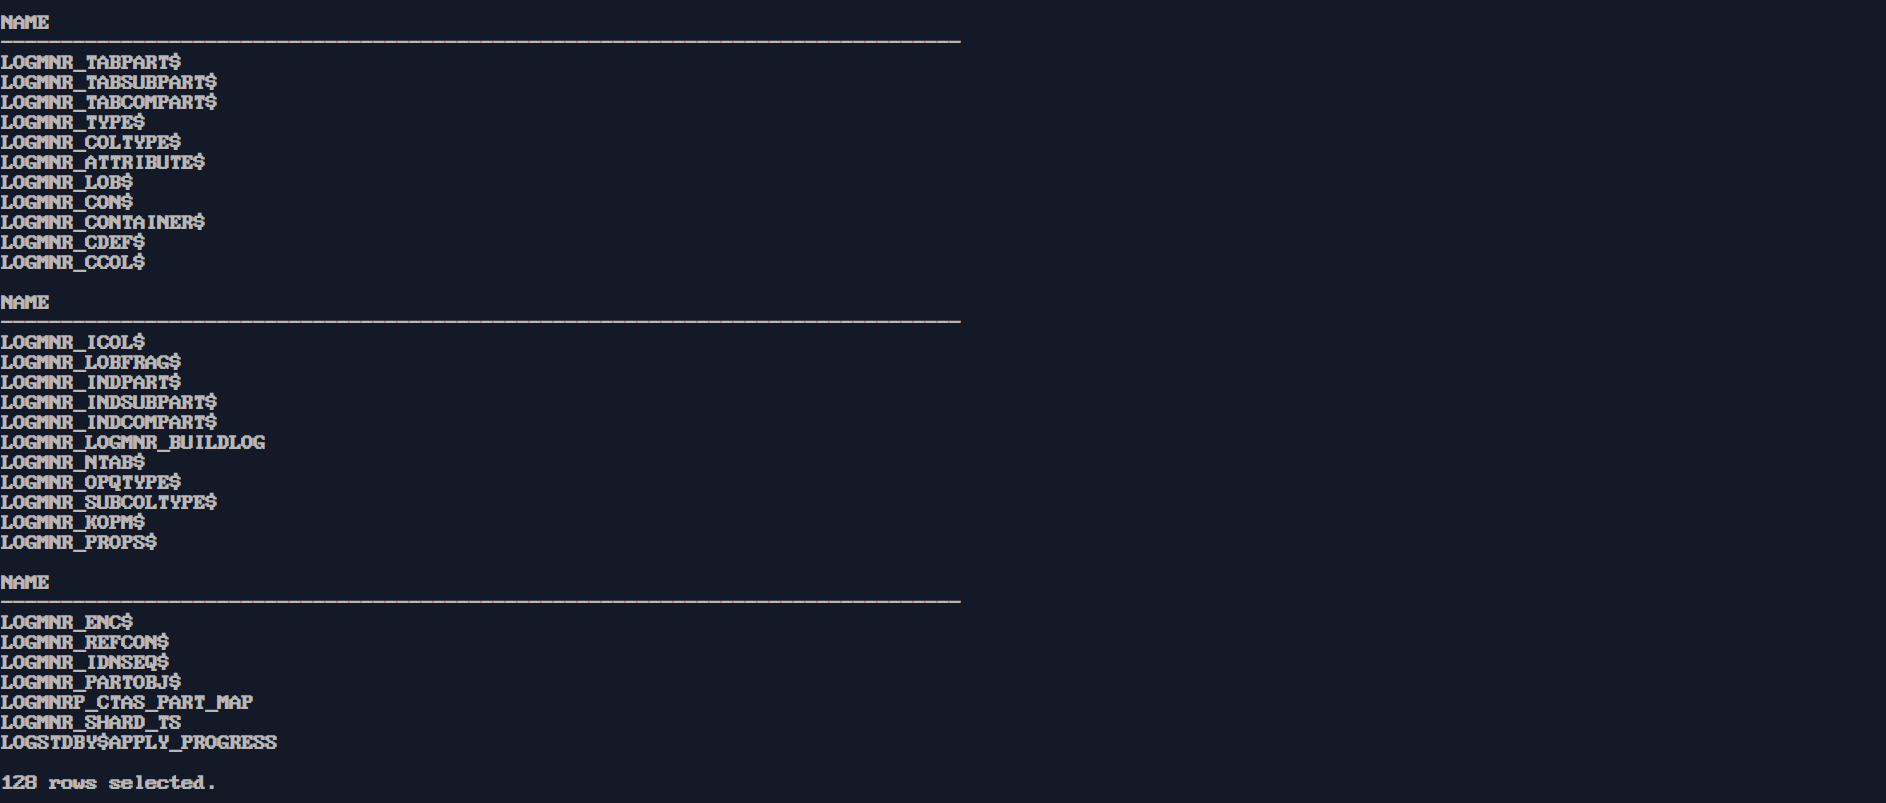
\includegraphics[width=\textwidth]{ScreenShot/Partie5/q6.a.png}
\end{center}


\subsubsection*{6.b}

\lstinputlisting[style=sqlstyle]{SQL/Partie5/q6.b.sql}

\begin{center}
    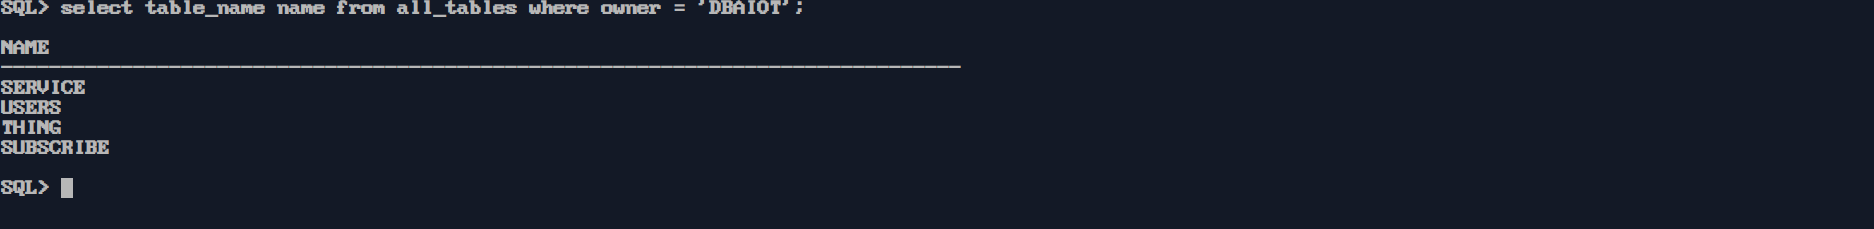
\includegraphics[width=\textwidth]{ScreenShot/Partie5/q6.b.png}
\end{center}

